\chapter{Эксперименты}

\section{Данные}
\indent В качестве экспериментальных данных использовалась база МРТ-снимков Alzheimer's Disease Neuroimaging Initiative. Данные содержат снимки пациентов в различными стадиями развития болезни Альцгеймера: 
\begin{enumerate}
    \item здоровые пациенты: NC (normal cohort)
    \item пациенты с умеренными когнитивными нарушениями: EMCI (early mild cognitive impairment)
    \item пациенты с выраженными когнитивными нарушениями: LMCI (late mild cognitive impairment)
    \item пациенты с болезнью Альцгеймера: AD (Alzheimer's disease)
\end{enumerate}

\indent Таким образом, решается задача классификации для четырех классов. \\
База данных состоит из снимков 228 пациентов, всего 748 снимков. Средний возраст испытуемых на момент начала эксперимента: $72.9 \pm 7.4$ лет. Среди пациентов 96 женщин и 132 мужчины. Распределение по классам следующее: 50 пациентов AD, 43 LMCI, 77 EMCI, 61 NC. \\
\indent T1-взвешенные снимки были обработаны с помощью FreeSurfer \cite{fischl2012freesurfer}. В обработке использовался атлас Desikan-Killiany \cite{desikan2006automated}, содержащий 68 регионов коры головного мозга. DWI (diffusion weighted imaging) снимки были скорректированы с учетом искажений, вызванных движением. Вероятностная трактография была выполнена с использованием модуля локального трекинга (LocalTrecking) фреймворка Dipy \cite{garyfallidis2014dipy} с ограничением на обратную сферическую свертку (constrained spherical deconvolution, CSD \cite{tax2014recursive}). Нервные связи длинее 5 мм, с обоих концов пересекающие поверхность коры, были удалены. Веса ребер графа, представляющего связность регионов, были высчитаны в соответствии с числом детектированых нервных связей.

\section{Влияние ранга матриц данных на результат классификации}
\indent В этом разделе рассматривается влияние ранга матриц данных на расстояния между ними и точность классификации. В частности, проверяется гипотеза о том, может ли искусственное снижение ранга повлиять на погрешность трактографии, допускаемую при исходной обработке МРТ-снимков.\\
\indent Для искусственного снижения ранга использовалось сингулярное разложение матриц $$\bx_i = U*S*V, \bx_i \in S^+(n,p),$$ где $S$ - диагональная матрица собственных значений $\bx_i$. Пусть $k \in \setN$ - ранг матрицы, который мы хотим получить после преобразования. Для снижения ранга заменяем $p-k$ минимальных собственных значений нулями: $$ S_{j,j} = 0, j \in \set{1, \ldots, p-k} $$
Можем видеть, что матрица расстояний меняется практически линейно в зависимости от ранга:
\begin{figure}[!h]
\minipage{0.32\textwidth}
  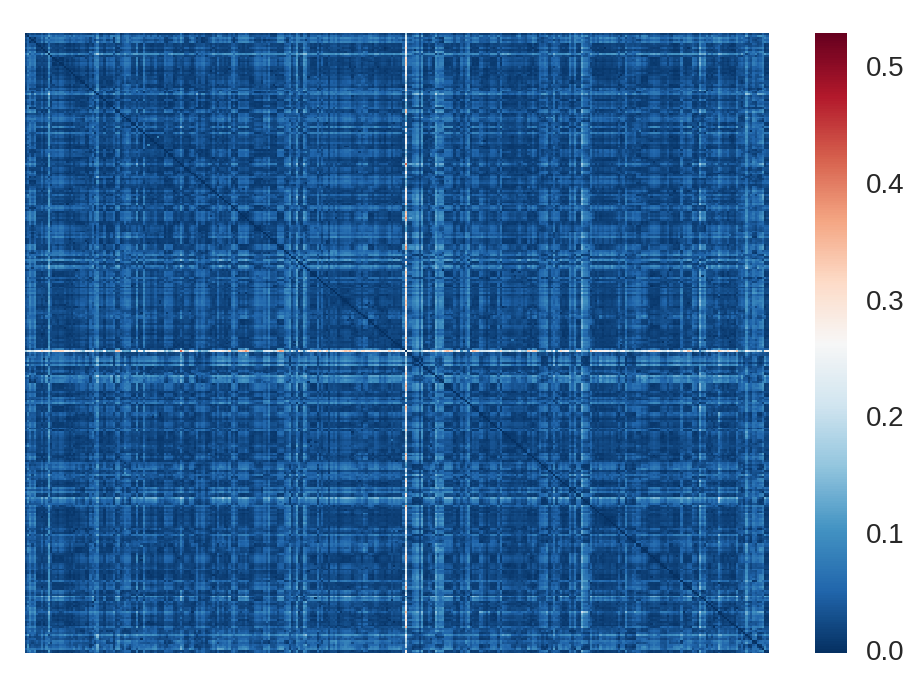
\includegraphics[width=\linewidth]{img/diff_drop_4.png}
  \caption{}
\endminipage\hfill
\minipage{0.32\textwidth}
  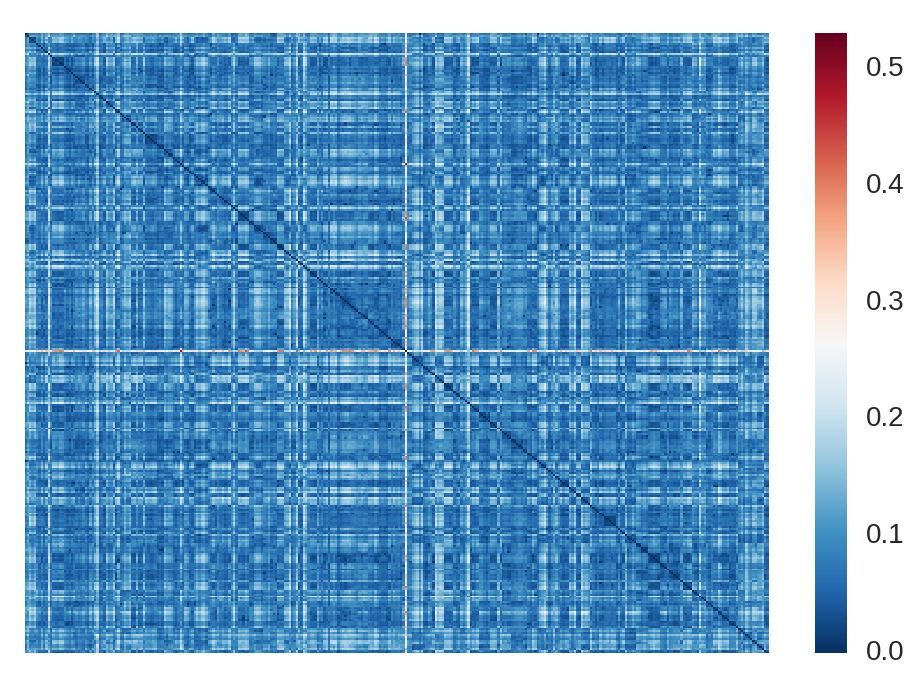
\includegraphics[width=\linewidth]{img/diff_drop_8.png}
  \caption{}
\endminipage\hfill
\minipage{0.32\textwidth}
  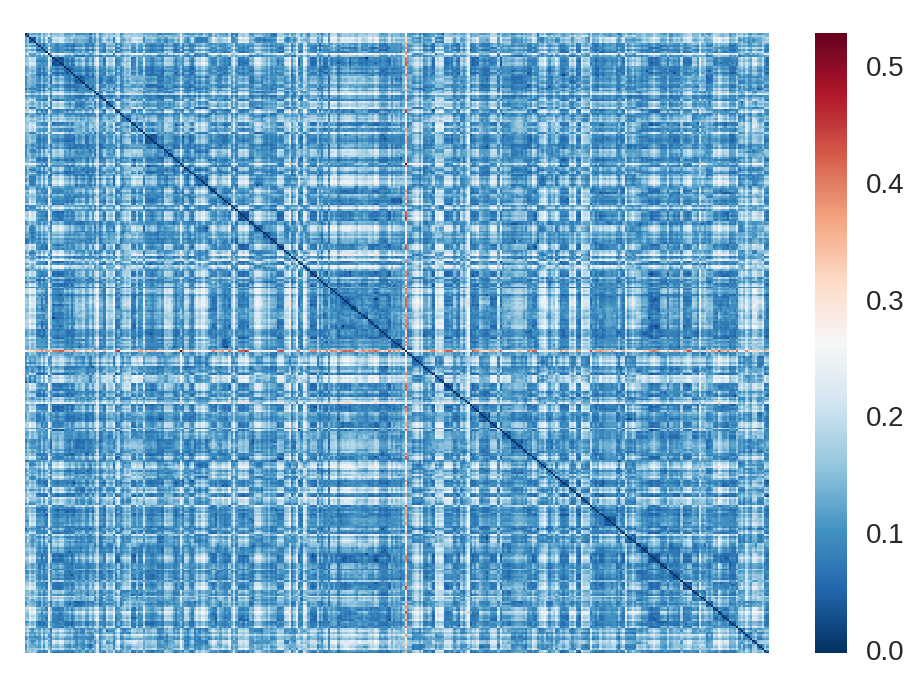
\includegraphics[width=\linewidth]{img/diff_drop_12.png}
  \caption{}
\endminipage
\caption{Изменение матрицы расстояний между матрицами данных при снижении ранга матриц данных на 4 (7.1), 8 (7.2) и 12(7.3)}
\end{figure}

\section{Базовые результаты}
\indent В качестве ориентировочных результатов использовались результаты двух методов:
\begin{enumerate}
    \item Как простейший метод, использовался алгоритм ядерной опорной машины векторов с ядром на основе $L2$ расстояний между матрицами данных
    \item Ядерный подход, предложенный в \cite{dodero2015kernel}. После высчитывания лапласианов матриц данных, к ним были добавлены единичные матрицы с коэффициентом $1e-3$ (алгоритм устойчив к выбору этого коэффициента, как предположено в \cite{dodero2015kernel}). Далее было высчитано логаримфированное евклидово расстояние между матрицами и классифицировано ядерным SVM с гауссовским ядром. Подробно алгоритм описан в \cite{dodero2015kernel}
\end{enumerate}

\section{Постановка эксперимента}
\indent В эксперименте проверялись результаты двух методов, предложенных прошлой главе:
\begin{enumerate}
    \item Ядерный SVM на основе «метрики» $\delta^k_{spsd}$
    \item Снижение размерности СППО матриц с помощью Isomap с последующей классификацией в пространстве меньшей размерности с помощью логистической регрессии с $l2$ регуляризацией.
\end{enumerate}

\begin{itemize}
    \item Для ядерных методов использовался поиск по множеству значений параметра $\gamma$ формулы \eqref{kernel} и параметру регуляризации $C$ машины опорных векторов.
    \item Для алгоритма Isomap использовался поиск по множеству значений итоговой размерности и числа соседей.
    \item Для логистической регрессии использовался поиск по параметру регуляризации.
    \item Для всех алгоритмов использовался поиск по значению коэффициента $k$ формулы \eqref{spsd-distance}
\end{itemize}
Поскольку в теоретических исследованиях не дается рекомендаций по выбору $k$ в \eqref{spsd-distance} \cite{bonnabel2009riemannian}, то выбор $k$ был произведен с помощью вычислительного эксперимента.
 
\indent Используемые множества значений параметров представлены в таблице ниже.\\
 
\begin{table}[!h]
\centering
\begin{tabular}{lll}
\hline
\rowcolor[HTML]{EFEFEF} 
Алгоритм                & Параметр                            & Множество значений                                                                                                                                                                                                        \\ \hline
Ядерные методы          & Коэффициент $\gamma$                & $\set{10^{0.25i}}_{i=-12}^4, \ i\in \setN$
     \\ 
Ядерные методы          & Параметр регуляризации SVM          & 0.1, 1, 5, 10, 50                                                                                                                                                                                                         \\
Isomap                  & Размерность итогового пространства  & 2, 4, 6, 8, 10                                                                                                                                                                                                            \\
Isomap                  & Число соседей                       & 60, 100, 150, 200, 250                                                                                                                                                                                                    \\
Логистическая регрессия & Параметр регуляризации              & $\set{10^{i}}_{i=-5}^3, \ i \in \setN $                                                                                                                                                                      \\
Все алгоритмы           & Коэффициент $k$ в $\delta_{spsd}^k$ & $\set{10^i}_{i=-4}^2, \ i \in \setN$ 
\end{tabular}
\caption{Множества значений параметров, использовавшиеся в переборе}
\end{table}

\indent Параметры были подобраны с использованием 10-фолдной кросс-валидации. В качестве алгоритма кросс-валидации использовался KFold, позволяющий гарантированно определять снимки одного пациента в один и тот же фолд. \\
Для лучших параметров кросс-валидация была повторена 10 раз на разных разбиениях данных, чтобы оценить эффективность алгоритмов.

\indent В качестве метрики качества во всех экспериментах использовалась площадь под ROC-кривой (ROC AUC)
\begin{definition}
\indent ROC-кривая – кривая, отображающая соотношение True positive rate и False positive rate при варьировании решающего правила классификатора
\end{definition}
\indent В интегральном выражении площадь под ROC-кривой задается следующим выражением:
\begin{equation}
\label{roc-auc}
    AUC =\int _{\infty }^{-\infty }{TPR}(T)\left(-FPR'(T)\right)\,dT=\int _{-\infty }^{\infty }\int _{-\infty }^{\infty }I(T'>T)f_{1}(T')f_{0}(T)\, \ dT'\,dT=P(X_{1}>X_{0})
\end{equation}

\indent Алгоритм построения ROC-кривой и явного вычисления ROC AUC представлен ниже\\
\begin{algorithm}[H]
    $m^- = \sum_{i=1}^n [y_i=-1]\;
    m^+ = \sum_{i=1}^n [y_i = +1]$\;
    $(FPR_0, \ TPR_0) = (0,0)$\;
    $AUC = 0$\;
    \For{$i=1, \ldots, N$}{
        \If{$y_i=-1$}{
            $FPR_i = FPR_{i-1}+\frac{1}{m^-}$\;
            $TPR_i = TPR_{i-1}$\;
            $AUC = AUC + \frac{1}{m^-}TPR_i$\;
        }
        \else{
            $FPR_i = FPR_{i-1}$\;
            $TPR_i = TPR_{i-1} + \frac{1}{m^+}$
        }
    }
\end{algorithm}
